\section{Conjecture sur l'erreur de généralisation}
\label{sec:appexp}

\begin{lemme}[Généralisation du lemme de Hoeffding]
  \label{b:lem:hoeffding}
  Ce lemme généralise le lemme de Hoeffding à un espace vectoriel de dimension arbitraire
  $\Q$. Soit un vecteur aléatoire $Q\in\Q$ tel que $\nq{Q}\leq\beta$ et $\E Q = 0$. Alors pour tout
  $t\in\Q$, 
  \begin{equation}
    \E e^{\inp{t,Q}} \leq \exp\left(\frac{\beta^2\|t\|^2}{2}\right).
  \end{equation}
  En effet, on sait que par définition de la convexité de la fonction exponentielle, pour
  tout $s\in[0,1]$,
  \begin{equation}
    \exp(sa + (1-s)b) \leq s\exp a + (1-s)\exp b.
  \end{equation}
  Donc en définissant $g:\{q \in \Q:\|q\|\leq\beta\}\to[0,1]$ par
  \begin{equation}
    g(q) = \frac{1}{2}\left(\frac{\inp{t,q}}{\beta\|t\|} + 1\right)
  \end{equation}
  et en posant $a = \beta\|t\|$ et $b = -\beta\|t\|$, alors pour tout $q \in \Q$,
  \begin{gather}
    a g(q) = \frac{1}{2}(\inp{t,q} + \beta\|t\|),\\
    b (1-g(q)) = - \frac{1}{2}(\beta\|t\| - \inp{t,q}),
  \end{gather}
  et donc
  \begin{equation}
    \exp(ag(q) + (1-g(q))b) = e^{\inp{t,q}}.
  \end{equation}
  La branche droite de l'inégalité devient quant à elle
  \begin{equation}
    \left(\frac{\inp{t,q}}{\beta\|t\|} + 1\right)e^{\beta\|t\|} + \left(1-\frac{\inp{t,q}}{\beta\|t\|}\right)e^{-\beta\|t\|}
  \end{equation}
  et donc, puisque $\E\inp{t,Q} = \inp{t,\E Q} = 0$, 
  \begin{align}
    \E e^{\inp{t,Q}} &\leq \E\left(\left(\frac{\inp{t,Q}}{\beta\|t\|} + 1\right)e^{\beta\|t\|} +
                       \left(1-\frac{\inp{t,Q}}{\beta\|t\|}\right)e^{-\beta\|t\|}\right)\\
                     &= e^{\beta\|t\|} + e^{-\beta\|t\|}\\
                     &= e^{\phi(\beta\|t\|)}
  \end{align}
  où $\phi(x) = \log(e^{x} + e^{-x})$. Or, avec le résultat de \cite{mohri2012foundations},
  p.~370, on a $\phi(x) \leq x^2/2$, d'où on tire le résultat annoncé.
\end{lemme}

\begin{lemme}[Généralisation de la borne de Chernoff]
  \label{b:lem:chernoff}
  Ce lemme généralise la borne de Chernoff à un espace vectoriel de dimension arbitraire
  $\Q$. Soit un vecteur aléatoire $Q \in \Q$. Alors l'évènement $\|Q\| \geq \epsilon$ aura lieu si et
  seulement s'il existe $t \in \Q$, $\|t\|=1$ tel que $\inp{t,Q} \geq \epsilon$. Ainsi, pour tout
  $s>0$, en employant l'inégalité de Markov, 
  \begin{align}
    \pp\{\|Q\| \geq \epsilon\} &= \pp\{s\inp{t,Q} \geq s\epsilon\} = \pp\{e^{s\inp{t,X}} \geq e^{s\epsilon}\}\\
                     &\leq e^{-s\epsilon}\E e^{\inp{t,Q}}.
  \end{align}
\end{lemme}

\begin{conj}[Généralisation de l'inégalité de McDiarmid]
  \label{b:lem:mcdiarmid}
  L'inégalité de McDiarmid peut également se généraliser à des fonctions prenant leurs
  valeurs dans des espaces vectoriels À élaborer!

  Soit une distribution $\mathscr{F}$ à valeur dans un espace quelconque $\bm F$, un
  espace vectoriel $\Q$ et une fonction $f:\bm F^n\to \Q$. S'il existe une constante
  $c\in\Re$ telle que pour deux ensembles d'échantillons \iid\ $\S_n \sim \mathscr{F}^n$ et
  $\S'_n$, où $\S_n$ et $\S'_n$ ne diffèrent que d'un seul point rééchantilloné de
  $\mathscr{F}$, on a
  \begin{equation}
    \|f(\S_n) - f(\S'_n)\| \leq c,
  \end{equation}
  alors pour tout échantillon aléatoire $\S_n\sim\mathscr{F}^n$, 
  \begin{equation}
    \pp\{\|f(\S_n) - \E f(\S_n)\| \geq \epsilon\} \leq \exp\left(-\frac{2\epsilon^2}{nc^2}\right).
  \end{equation}
\end{conj}


\begin{conj}[Borne sur la décision]
  \label{b:lem:qhnorm}
  Considérons le cas d'une utilité neutre au risque puisqu'on sait que toute solution à
  $\max_q\EU_\lambda(q)$ sera bornée par celle de $\max_q\EN_\lambda(q)$.  La stabilité de
  l'algorithme $\alg$ fournie par \cite{bousquet2002stability} établit que pour deux
  échantillons $\S_n$ et $\S_n'$ tirés de $M^n$ et ne différant que d'un seul point,
  \begin{equation}
    \|\alg(\S_n) - \alg(\S'_n)\| \leq \frac{\rmax\xi}{\lambda n}.
  \end{equation}
  En posant $\qh \sim \alg(M^n)$, on peut donc appliquer directement le résultat de
  l'inégalité de McDiarmid (\lemref{b:lem:mcdiarmid}) pour obtenir avec probabilité
  $1-\delta$ que
  \begin{equation}
    \|\qh - \E\alg(\S_n)\| \leq \frac{\rmax\xi}{\lambda}\sqrt{\frac{\log(1/\delta)}{2n}}.
  \end{equation}
  Or, $\alg$ est un estimateur non-biaisé de $\qsl$. En effet, pour une utilité neutre au
  risque,
  \begin{align}
    \E\alg(\S_n) &= \E_{M^n}\left(\frac{1}{2n\lambda}\sumi r_i\,\kappa(\cdot,x_i)\right)\\
                 & =\frac{1}{n}\sumi \frac{1}{2\lambda}\E_M(R\,\kappa(\cdot,X))\\
                 & =\frac{1}{n}\sumi \qsl\\
                 &=\qsl.
  \end{align}
  On obtient ainsi
  \begin{equation}
    \|\qh - \qsl\| \leq \frac{\rmax\xi}{\lambda}\sqrt{\frac{\log(1/\delta)}{2n}}.
  \end{equation}
\end{conj}

\begin{conj}
  Pour tout ensemble d'entraînement $\S_n$, on a
\begin{equation}
  |\hat\zeta_u(\S_n)| \leq |\hat\zeta_1(\S_n)|.
\end{equation}
où $\hat\zeta_u$ est l'erreur de généralisation en employant une fonction d'utilité quelconque
et $\hat\zeta_1$ l'erreur de généralisation avec une attitude risque neutre.
\end{conj}

\begin{rem}
  Il est probable que la preuve soit simplement un argument de forte convexité dûe à la
  régularisation, mais aussi un phénomène plus complexe comme une généralisation
  multivariée de l'inégalité de Jensen.
\end{rem}

\begin{conj}
  On a, avec probabilité $1-\delta$ sur l'échantillonage de l'ensemble d'entraînement $\S_n$, 
  \begin{equation}
    \hat\zeta_1(\S_n) \leq \frac{\rmax^2\xi^2}{\lambda}\sqrt\frac{\log(1/\delta)}{2n}.
  \end{equation}
\end{conj}

\begin{proof}
  On a la chaîne d'inégalités suivantes:
  \begin{align}
    \hat\zeta_1(\qh) &= \hEN(\qh) - \EN(\qh)\\
                 &= \langle\hEN - \EN|\qh\rangle\\
                 &= \lambda\langle\qh - \qsl|\qh\rangle\\
                 &\leq \lambda\|\qh - \qsl\|\|\qh\|\\
                 &\leq \frac{\rmax^2\xi^2}{\lambda}\sqrt\frac{\log(1/\delta)}{2n}
  \end{align}
  en utilisant les résultats de la Conjecture \ref{b:lem:qhnorm} et du Lemme
  \ref{lem:ndef}.
\end{proof}

\begin{figure}[p]
  \centering
  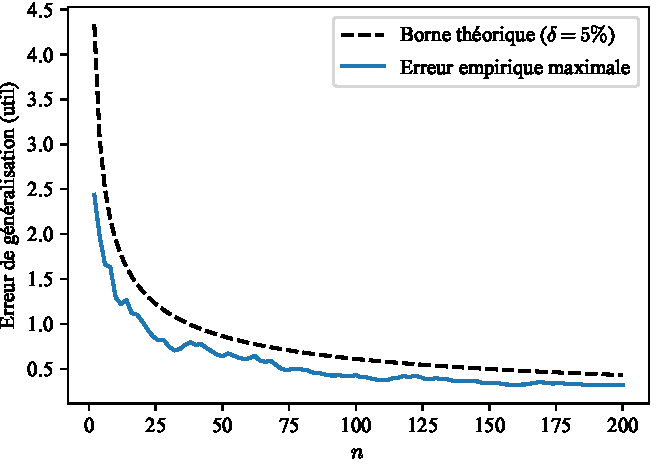
\includegraphics[width=\textwidth]{../experiments/fig/conjec.pdf}
  \caption[Erreur de généralisation -- Conjecture]
  {Progression de l'erreur maximale de généralisation sur $m=150$ ensembles
    d'entraînement et $p=5$. On constate que la borne théorique issue de la conjecture de
    l'Annexe \ref{sec:appexp} est \textsl{beaucoup} plus serrée que les figures
    dérivées à partir des Théorèmes 1 et 2.}
  \label{fig_conjec}
\end{figure}


%%% Local Variables:
%%% mode: latex
%%% TeX-master: "memoire"
%%% End:
